\section{Mecânicas de jogo}

\subsection{Fase 1 - MVP}
O jogador se movimenta pela Torre PontiAguda selecionando
um dos nós mais próximos de sua posição atual, como no 
jogo \textit{Slay The Spire}, e avança para essa nova 
posição se vencer o confronto ou realizar uma ação 
disponível nesse nó.

Durante o combate, o jogador seleciona algumas espadas 
para se conectar e energizar com uma quantidade finita 
de mana, permitindo que elas realizem ações 
específicas durante o combate.

A mana é um recurso finito que precisa ser gerenciado pelo 
jogador, podendo ser obtida dos inimigos derrotados, 
por meio de pedras de mana e meditação em lugares 
específicos.

As espadas têm efeitos e ataques individuais. Além disso,
podem se combinar com outras espadas para evoluir, como em 
\textit{Backpack Battles}.


\subsection{Fase 2 - Versão Final}
O jogador poderá mover seu personagem usando WASD, buscar
oponentes pelo mapa para desafiá-los, os quais poderão ou 
não aceitar os desafios, e ser desafiado por oponentes 
aleatórios no mapa. 

Os desafios serão aceitos ou recusados com base na 
estimativa da quantidade de mana do oponente feita por 
cada personagem.

As espadas companheiras poderão ficar flutuando em torno 
do jogador para interagir com o ambiente ou permanecer na
mão do jogador para serem usadas em combate contra 
criaturas sem espadas em ruínas.

Para acessar a Torre PontiAguda, o jogador precisará
explorar ruínas ao redor da Torre para encontrar os 
símbolos espirituais, que liberam acesso às habilidades 
de uma \textit{skill tree}, como a de \textit{Arc Raiders}
, o que traz maior variedade ao jogo.


\begin{figure}[!ht]
    \centering

    \begin{subfigure}{0.3\textwidth}
        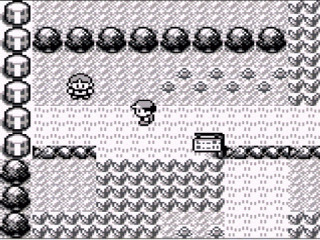
\includegraphics[width=\textwidth]{images/pokemon_sample_2.jpg}
        \caption{Pokémon visão \textit{top-down}}
        \label{fig:pokémon_top-down}
    \end{subfigure}
    \hspace{0.6cm}
    \begin{subfigure}{0.4\textwidth}
        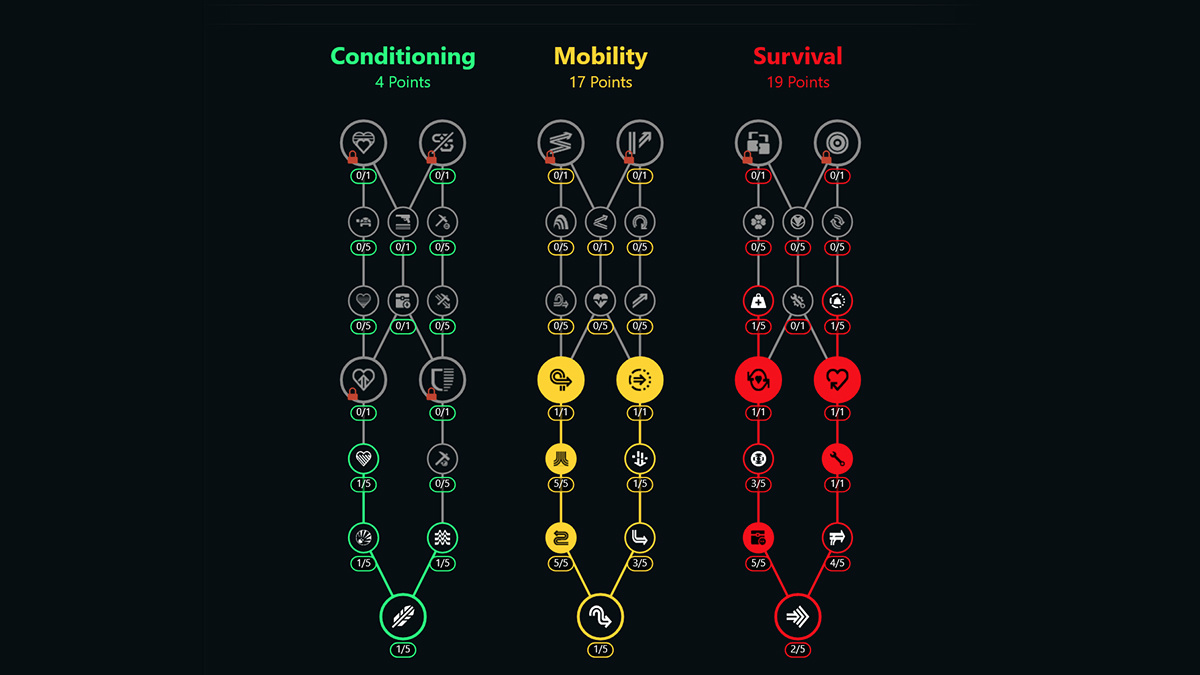
\includegraphics[width=\textwidth]{images/arc_raiders_skill_tree.jpg}
        \caption{\textit{Arc Raiders Skill Tree}}
        \label{fig:skill_tree_sample}
    \end{subfigure}

    \caption{Imagens de referência para as mecânicas da fase 2}
    \label{fig:imagens_referencia_mecanics_final}
\end{figure}
